
The so-called Granovetter-Watts model was introduced to capture a situation in which the adoption of new ideas or technologies requires a certain redundancy in the social environment of each agent to take effect. This model has become a paradigm for complex contagion. Here we investigate a symmetric version of the model: agents may be in two states that can spread equally through the system via complex contagion. We find three possible phases: a mixed one (dynamically active disordered state), an ordered one, and a heterogeneous frozen phase. These phases exist for several configurations of the contact network. Then, we consider the effect of introducing aging as a non-Markovian mechanism in the model, where agents become increasingly resistant to change their state the longer they remain in it.  We show that when aging is present, the mixed phase is replaced, for sparse networks, by a new phase with different dynamical properties. This new phase is characterized by an initial disordering stage followed by a slow ordering process towards a fully ordered absorbing state. In the ordered phase, aging modifies the dynamical properties. For random contact networks, we develop a theoretical description based on an Approximate Master Equation that describes with good accuracy the results of numerical simulations for the model with and without aging.
	
\section{\label{sec:Introduction} Introduction}
	
In recent decades, various techniques of probability and statistical physics have been employed to measure and explain social phenomena \cite{castellano2009statistical,jusup2022social,bianconi2023complex}. A variety of social collective phenomena can be well understood through stochastic binary-state models of interacting agents. In these models, each agent is assumed to be in one of two possible states, such as susceptible/infected, adopters/non-adopters, etc., depending on the context of the model. The interaction among agents is determined by the underlying contact network and the dynamical rules of the model. There are various examples of binary-state models, including processes of opinion formation \cite{Voter-original, sood-2005, Suchecki-2005, fernandez-gracia-2014, redner-2019} and disease or social contagion \cite{granovetter-1978, pastor-satorras-2015}, among others. The consensus problem consists of determining under which circumstances the agents end up sharing the same state or when the coexistence of both states prevails. This is characterized by a phase diagram that provides the boundaries separating domains of different behaviors in the control parameter space. Macroscopic descriptions of these models in terms of mean-field, pair, and higher-order approximations are well established \cite{gleeson-2011}. 
	
An important category of binary-state models are threshold models \cite{watts-2002}, which were originally introduced by M. Granovetter \cite{granovetter-1978} to address problems of social contagion such as rumor propagation, innovation adoption, riot participation, etc. Multiple exposures, or group interaction, are necessary in these models to update the current state, a characteristic of complex contagion models \cite{centola-2007,unknown-author-2018}. The threshold model presents a discontinuous phase transition from a ``global cascade'' phase to a ``no cascade'' phase, which was analyzed in detail in Ref. \cite{watts-2002}. This model has been extensively studied on various network topologies, such as regular lattices, small-world \cite{centola-2007}, random \cite{gleeson-2007}, clustered \cite{hackett-2011,hackett-2013}, modular \cite{gleeson-2008}, hypergraphs \cite{de-arruda-2020}, homophilic \cite{diaz-diaz-2022} and coevolving \cite{min2023threshold} networks. 
	
A main difference between the threshold model and other binary-state models, such as the Voter \cite{Voter-original}, majority vote (MV) \cite{de1992isotropic,pereira2005majority,campos2003small}, and nonlinear Voter model \cite{castellano-2009,mobilia2015nonlinear,mellor2016characterization,Min-2017,jewski-2017,peralta-2018}, is the lack of symmetry between the two states. In the threshold model, changing state is only possible in one direction, representing the adoption forever of a new state that initially starts in a small minority of agents. A symmetric version of the threshold model, with possible changes of states in both directions, was introduced in Refs. \cite{nowak2019homogeneous,nowak2020symmetrical} to investigate the impact of noise and anticonformity. However, a complete characterization of the Symmetrical Threshold model and its ordering dynamics have not been addressed so far.

\section{\label{Symmetrical Threshold model} Symmetrical Threshold model}

%The interaction dynamics of the Symmetrical Threshold model are motivated by the threshold model introduced by M. Granovetter \cite{granovetter-1973}. While the original binary-state model only considers the propagation of one state through the system (asymmetric model), in this study we consider the symmetric case, where both states are allowed to propagate. 
The system consists of a set of $N$ agents located at the nodes of a network. The variable describing the state of each agent $i$ takes one of the two possible values: $s_i = \pm 1$. Every agent has assigned a fixed threshold $0 \leq T \leq 1$, which determines the fraction of different neighbors required to change state. Even though this value might be agent-dependent, we will consider here only the case with a homogeneous $T$ value for all the agents of the system. In each update attempt, an agent $i$ (called active agent) is randomly selected, and if the fraction of neighbors with a different state is larger than the threshold $T$, the active agent changes state $s_i \to -s_i$. In other words, if $m$ is the number of neighbors in state $-1$ out of the total number of neighbors $k$, the condition to change is $\theta(m/k - T)$, for a node in state $+1$, and $\theta((k-m)/k - T)$, for a node in state $-1$, where $\theta(x)$ is the Heaviside step function. Notice that this update rule is equivalent to ``shifted'' Glauber dynamics \cite{glauber1963time}, with swapping probability $1/(1+\exp[\beta(\Delta E + C)]$ (where $\beta$ is the inverse temperature, $\Delta E$ the energy loss to swap the state of a node according to Ising Hamiltonian and $C$ a shifting constant), at the limit of zero temperature ($\beta \to \infty$). We analyze the model dynamics using numerical simulations. Simulation time is measured in Monte Carlo (MC) steps, i.e., $N$ update attempts. Numerical simulations run until the system reaches a frozen configuration (absorbing state) or until the average magnetization, $m = (1/N) \sum_i s_i$, fluctuates around a constant value.

\section{\label{sec:Dynamics on networks} Dynamics on networks}

\subsection{Mean-field}

\begin{figure}
	\centering \captionsetup{font=sf}
	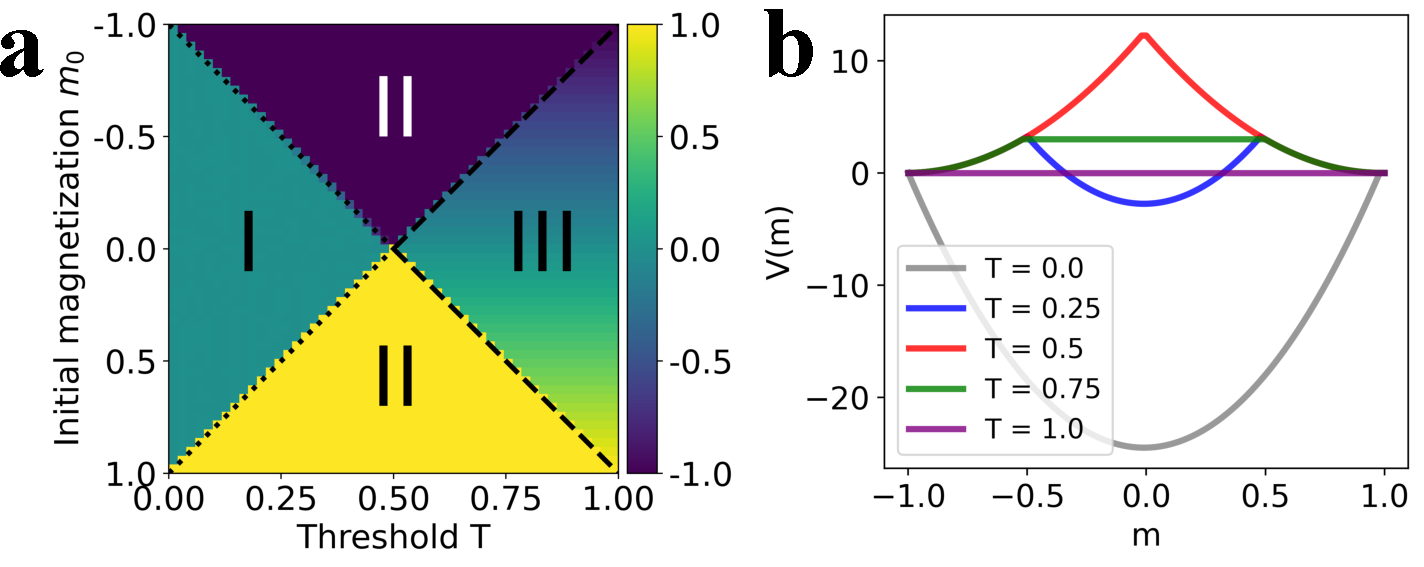
\includegraphics[width=0.9\textwidth]{Figs/Aging_STM/FIG1.pdf}
	\caption[Phases of the Symmetrical Threshold model]{\textbf{(a)} Phase diagram of the Symmetrical Threshold model in a Complete graph of $N = 2500$ nodes. Dotted and dashed lines correspond to $T = (1-|m_0|)/2$ and $T = (1+|m_0|)/2$, respectively. Average performed over 5000 realizations. \textbf{(b)} Potential representation from Eq. (\ref{eq:potential}) for a set of values of the threshold $T$, shown in different colors.}
	\label{COM_LAT_PD}
\end{figure}

We first consider the mean-field case of the complete graph (all-to-all connections). We take an initial random configuration with magnetization $m_0$ and run numerical simulations for various values of $T$ to construct the phase diagram (shown in Fig. \ref{COM_LAT_PD}a). We find three different phases based on the final state:
\pagebreak
\begin{itemize}
	\item \textbf{Phase I or Mixed}: The system reaches an active disordered state (final magnetization $m_f = 0$) where the agents change their state continuously;
	\item \textbf{Phase II or Ordered}: The system reaches the ordered absorbing states ($m_f = \pm 1$) according to the initial magnetization $m_0$;
	\item \textbf{Phase III or Frozen}: The system freezes at the initial random state $m_f = m_0$.
\end{itemize}

For a given initial magnetization $m_0 \neq 0$ and increasing $T$, the system undergoes a mixed-ordered transition at a critical threshold $T_{c} = (1-|m_0|)/2$, and an ordered-frozen transition at a critical threshold $T_{c}^{*} = (1 + |m_0|)/2 > T_{c}$ (indicated by dotted and dashed black lines in Fig. \ref{COM_LAT_PD}a, respectively). In this mean-field scheme, if the fraction of nodes in state $+1$ is denoted by $x$, the condition for a node in state $-1$ to change its state is given by $\theta(x - T)$, where  $\theta$ is the Heaviside step function. Thus, in the thermodynamic limit ($N\to \infty$), the variable $x$ evolves over time according to the following mean-field equation:<
\begin{equation}
	\frac{dx}{dt} = (1 - x) \; \theta(x - T) - x \; \theta(1 - x - T) = - \frac{\partial V(x)}{\partial x}.
\end{equation}
Here, $V(x)$ is the potential function. The stationary value of $x$, $x_{\rm st}$, is the solution of the implicit equation resulting from setting the time derivative equal to $0$. The stationary solutions are $x_{\rm st} = 1/2$ ($m =0$), the absorbing states $x_{\rm st} = 0,1$ ($m = \pm 1$) or a degenerate continuum of solutions. The stability of these solutions can be understood in terms of the potential $V(x)$:
\begin{eqnarray}
	\label{eq:pot}
	V(x) &=-\int (1 - x) \; \theta(x - T) - x \; \theta(1 - x - T) \; dx \nonumber\\
	&=\frac{x^2}{2} + \frac{1}{2} \left( T^2 - 2T - x^2 + 1\right) \; \theta(T+x-1)\\
	&- \frac{1}{2} \left( T^2 - 2T - x(x-2)\right) \; \theta(x - T)\nonumber
\end{eqnarray}
The minimum and maximum values of $V(x)$ correspond to stable and unstable solutions, respectively. Figure \ref{COM_LAT_PD}b shows the potential's dependence on the magnetization, obtained after a variable change $m = 2x-1$ in Eq. (\ref{eq:pot}). For $T < 0.5$, $m = 0$ is a stable solution, but increasing the threshold reduces the range of values of the initial magnetization from which this solution is reached, enclosing Phase I between the unstable solutions $m = 1-2\, T$ and $2\, T-1$. In fact, if $m_0 > 1-2\, T$, the system reaches the absorbing solution $m=+1$, while if $m_0 < -1+2\, T$, it reaches $m=-1$ (Phase II). For $T = 0.5$, there is just one unstable solution at $m=0$, and all the initial magnetization values reach the absorbing states $m=\pm 1$. For $T > 0.5$, the potential is equal to a constant value for a range of $m_0$, which means that an initial condition will remain in this state forever (Phase III). The range of values of the initial condition from which this phase is reached grows linearly with $T$ until $T=1$, where all initial conditions fulfill $\frac{dm}{dt}=0$.

\begin{figure}
	\centering \captionsetup{font=sf}
	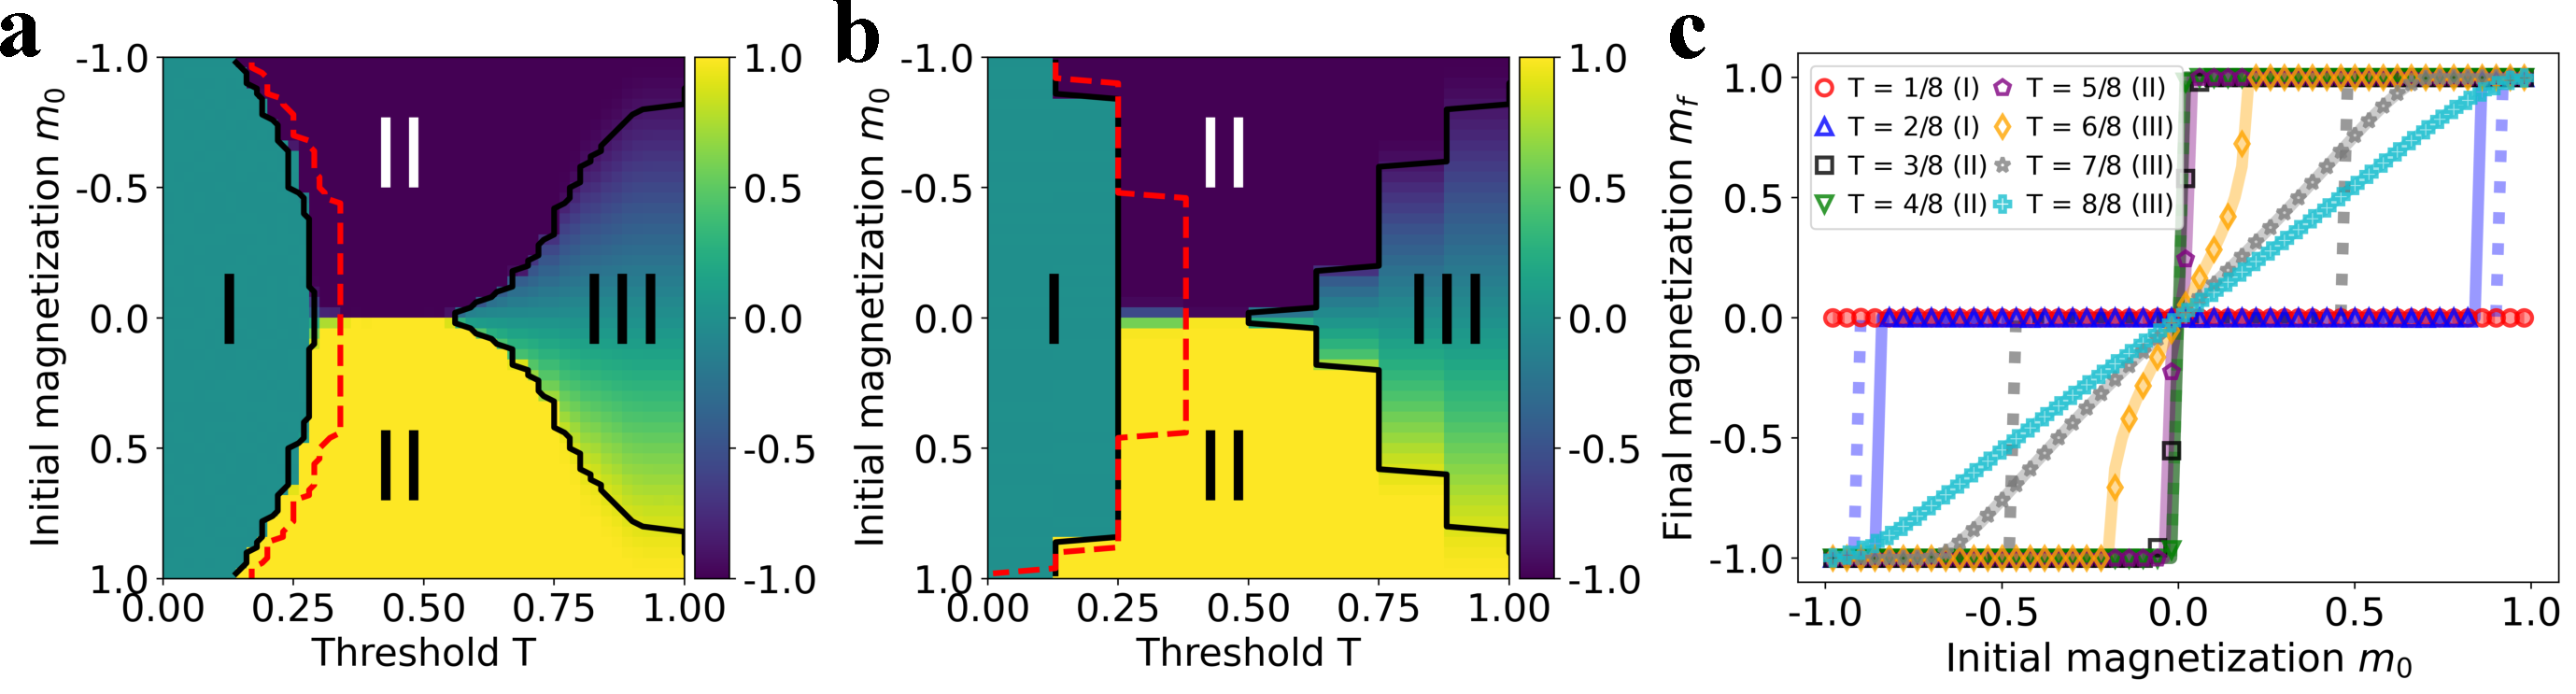
\includegraphics[width=\linewidth]{Figs/Aging_STM/FIG2.pdf}
	\caption[Phase diagram in random networks]{\label{ER_REG_PD} Phase diagram of the Symmetrical Threshold model in an ER \textbf{(a)} and a RR \textbf{(b)} graph, both of $N=4\cdot10^4$ nodes and mean degree $\langle k \rangle=8$. The color map indicates the value of the average final magnetization $m_f$. The red dashed line is the HMF prediction of the mixed-ordered critical line. The black solid lines correspond to the AME prediction of the borders of Phase II. \textbf{(c)} Average final magnetization $m_f$ as a function of the initial magnetization $m_0$ for different $T$ values (indicated with different colors and markers) in the RR graph. The average is performed over 5000 realizations. The dotted and solid lines are the HMF (for $T=1/8 - 4/8$) and AME predictions (for all $T$), respectively.}
\end{figure}


Note that the mean-field Symmetrical Threshold model for $T=1$ shows the same potential profile as the mean-field Voter model \cite{Suchecki-2005, Voter-original, Voter}. The important difference is that for the Voter model, any initial magnetization is marginally stable, while in our model any initial magnetization is an absorbing state in Phase III. In the Voter model finite size fluctuations will take the system to the absorbing states $m=\pm 1$. 

%The description is simple: If $T > 1/2$, the two conditions to reach order are $\pm m_0 > 2T - 1$. Note that if one of these conditions is true, the other is necessary false, describing the two symmetrical absorbing states $m_f =\pm 1$ (ordered phase). Contrary, if none of them are full-filed, the dynamics get frozen at the initial state because no updates are possible (frozen phase). If $T < 1/2$, the conditions $\pm m_0 > 2T - 1$ are not exclusive. When both conditions are fulfilled, the system exhibits the mixed phase (mixed phase). The system will only reach order when one condition is full-filed and the other one is not, what describes the both absorbing states, each one for each condition (ordered phase). For $T = \frac {1}{2}$ and $m_0 = 0$, we recover the majority vote MV model. In this situation, as a stochastic effect, the absorbing state may be $m_f = 1$ or $m_f = -1$.

\subsection{Random networks}

We analyze the phase diagram of the Symmetrical Threshold model in two random networks: Erd\H{o}s-Rényi (ER) \cite{erdos1960evolution} and random regular (RR) \cite{wormald1999models} graphs with mean degree $\langle k \rangle = 8$. Figures \ref{ER_REG_PD}a and \ref{ER_REG_PD}b show the phase diagram for both networks, where it is shown that the existence of the three phases previously described is robust to changes in network structure. The main difference from the all-to-all scenario is that Phase III does not freeze exactly at the same initial magnetization. Instead, the system reaches an absorbing state with a higher magnetization $m_f > m_0$. In this phase, the value of $m_f$ depends on the threshold such that increasing $T$, increases the disorder in the system, until $T = 1$, where $m_f = m_0$ (see Fig. \ref{ER_REG_PD}c). On the other hand, phases I and II reach the same stationary state as in the mean-field case. Furthermore, the critical thresholds $T_{c}$ and $T_{c}^{*}$ show a different dependence on $m_0$ depending on the network structure.

To explain the transitions exhibited by the model, we use a theoretical framework for binary-state dynamics in complex networks \cite{gleeson-2013}: the Approximate Master Equation (AME), which considers agents in both states $\pm 1$ with degree $k$, $m$ neighbors in state $-1$ that have been $j$ time steps in the current state (called ``internal time'' or ``age'') as different sets in a compartmental model (see details of the AME derivation in \cite{Abella-2022-AME,gleeson-2013}). In general, the AME is:
\begin{eqnarray}
	\label{eq:AME_age}
	\frac{d}{d t} x^{\pm}_{k, m, 0}(t)=&- x^{\pm}_{k, m, 0}(t) + \sum_l T^{\mp}_{k, m,l} \, x^{\mp}_{k, m, l}(t) - (k-m) \,\beta^{\pm} \, x^{\pm}_{k, m, 0}(t) - m \,\gamma^{\pm} \, x^{\pm}_{k, m, 0}(t), 
	\nonumber\\
	\frac{d}{d t} x^{\pm}_{k, m, j}(t)=&- x^{\pm}_{k, m, j}(t)+ A^{\pm}_{k, m,j} \, x^{\pm}_{k, m, j-1}(t) - (k-m) \,\beta^{\pm} \, x^{\pm}_{k, m, j}(t) + (k-m+1) \,\beta^{\pm} \, x^{\pm}_{k, m-1, j-1}(t)\nonumber\\
	&+ (m+1) \,\gamma^{\pm} \, x^{\pm}_{k,m+1,j-1}(t) - m \,\gamma^{\pm} \, x^{\pm}_{k, m, j}(t), \nonumber
\end{eqnarray}
where variables $x^{+}_{k,m,j}(t)$ and $x^{-}_{k,m,j}(t)$ are the fractions of $k$-degree nodes that are in state $+1$ (respectively, $-1$), have $m$ neighbours in state $-1$, and have age $j$. The configuration-dependent rates $\beta^{\pm}$ account for the change of state of neighbors ($\pm$) of a node in state $+1$. The rates $\gamma^{\pm}$ are equivalent but for nodes in state $-1$. To build the AME, we need to assume that these rates are equal for all nodes in the same state, as in Ref \cite{gleeson-2013}:
\begin{eqnarray}
	\beta^{+} = \frac{\sum_j \sum_k p_k \sum_{m = 0}^{k} (k - m) \, T^{+}_{k,m,j} \, x^{+}_{k,m,j}}{\sum_j \sum_k p_k \sum_{m = 0}^{k} (k - m) \, x^{+}_{k,m,j}}, \nonumber\\
	\beta^{-} = \frac{\sum_j \sum_k p_k \sum_{m = 0}^{k} m \, T^{+}_{k,m,j} \, x^{+}_{k,m,j}}{\sum_j \sum_k p_k \sum_{m = 0}^{k} m \, x^{+}_{k,m,j}},\nonumber\\
	\gamma^{+} = \frac{\sum_j \sum_k p_k \sum_{m = 0}^{k} (k - m) \, T^{-}_{k,m,j} \, x^{-}_{k,m,j}}{\sum_j \sum_k p_k \sum_{m = 0}^{k} (k - m) \, x^{-}_{k,m,j}},\\
	\gamma^{-} = \frac{\sum_j \sum_k p_k \sum_{m = 0}^{k} m \, T^{-}_{k,m,j} \, x^{-}_{k,m,j}}{\sum_j \sum_k p_k \sum_{m = 0}^{k} m \, x^{-}_{k,m,j}},\nonumber
\end{eqnarray}
	where the degree distribution of the chosen network is $p_k$. Notice that these equations are written using a dimensionless time $t$. The transition rate $T^{\pm}_{k,m,j}$ is for the probability of changing state ($\pm \to \mp$) for an agent of degree $k$, $m$ neighbors in state $-1$ and age $j$, while the aging rate $A^{\pm}_{k,m,j}$ is for the probability of staying in the same state and increasing the internal time ($j \to j + 1$). For the Symmetrical Threshold model, according to the update rules these rates do not depend on internal time $j$ (Markovian dynamics):
\begin{equation}
	T^{+}_{k,m,j} = \theta(m/k - T) \quad \quad T^{-}_{k,m,j} = \theta((k-m)/k - T) \quad \quad A^{\pm}_{k,m,j} = 1 - T^{\pm}_{k,m,j}.
\end{equation}
Therefore, if we were not concerned with the internal time dynamics, we can simplify our AME to the one proposed by J. P. Gleeson in Ref. \cite{gleeson-2013} for general binary-state models. Here we keep the internal times for a dynamical characterization of the different phases and as a reference frame for the aging studies in the next section. 

\begin{figure}
	\centering \captionsetup{font=sf}
	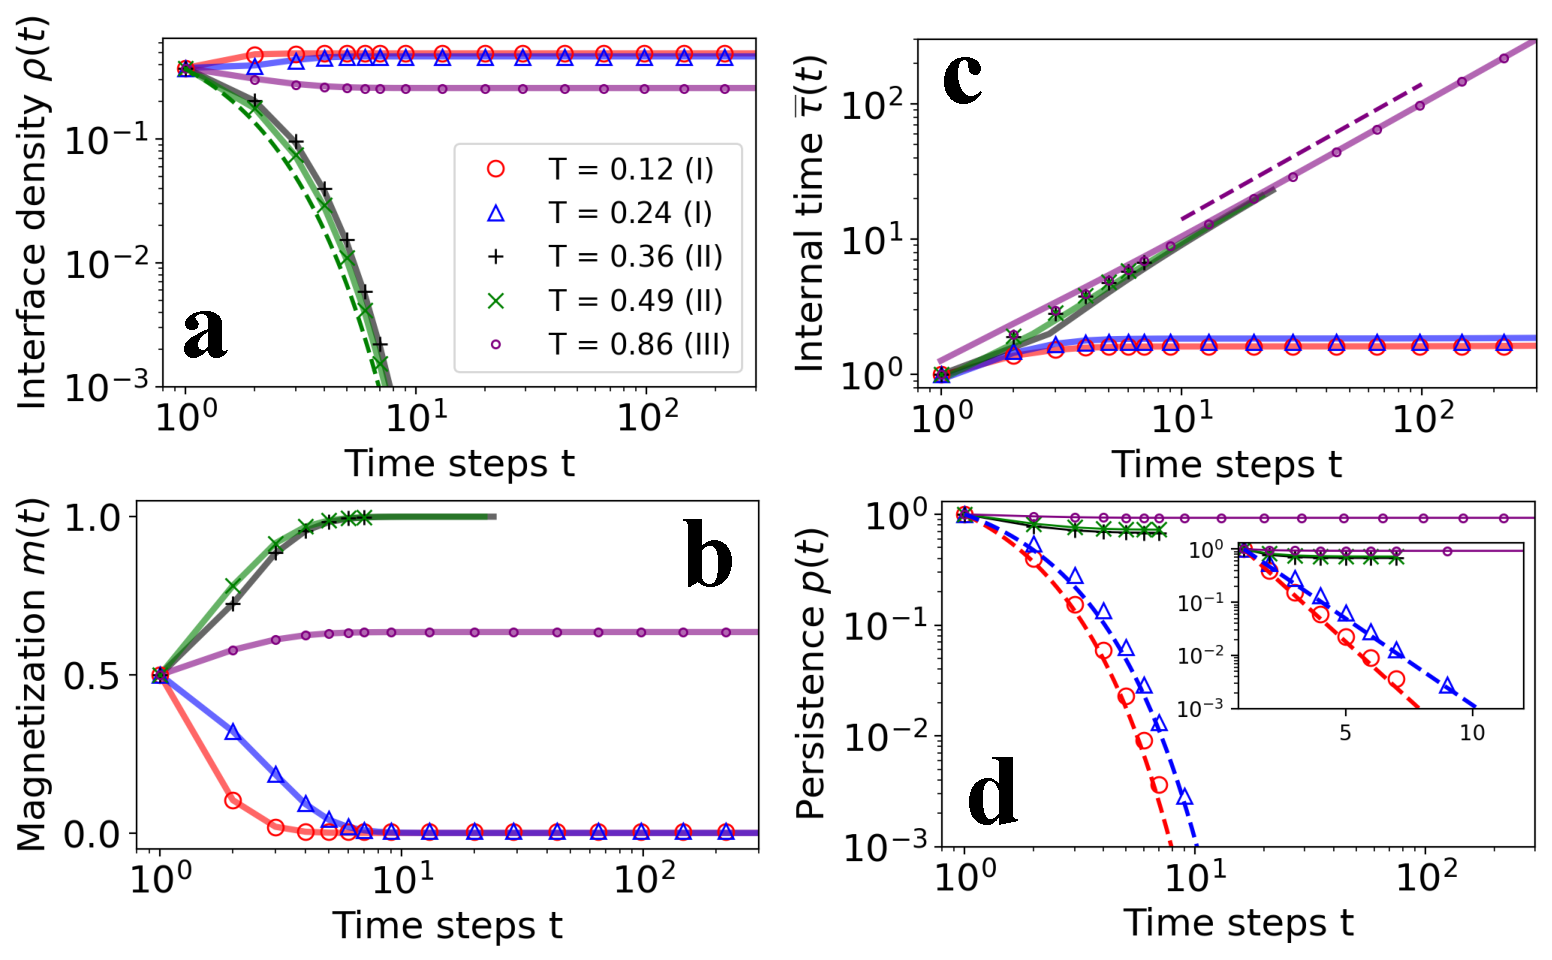
\includegraphics[width=\textwidth]{Figs/Aging_STM/FIG3.pdf}
	\caption[Symmetrical Threshold model dynamics in random networks]{\label{fig:evolution_random} Evolution of the average interface density $\rho(t)$ \textbf{(a)}, the average magnetization $m(t)$ \textbf{(b)}, the mean internal time $\bar{\tau}(t)$ \textbf{(c)}, and the persistence $p(t)$ \textbf{(d)} for the Symmetrical Threshold model. The average is computed over $5000$ surviving trajectories (simulations stop when the system reaches the absorbing ordered states). Results for different values of $T$ are plotted with diverse markers and colors: red ($T = 0.12$) and blue ($T = 0.24$) belong to Phase I, green ($T = 0.36$) and grey ($T = 0.49$) belong to Phase II and purple ($T = 0.86$) belongs to Phase III. Solid colored lines are the AME integrated solutions, using Eqs. (\ref{eq:interface})-(\ref{eq:time}). The initial magnetization is $m_0 = 0.5$. The system is on an ER graph with $N = 4 \cdot 10^4$ and mean degree $\langle k \rangle = 8$. The dashed green line in (a) shows $\rho(t) \sim \rho_0 \, e^{-t}$, the dashed purple line in (c) shows $\bar{\tau}(t) = t$ and the dashed lines in (d) show $p(t) \sim e^{-\alpha t}$, where $\alpha = 1$ (red) and $\alpha = 3/4$ (blue) 
	%(these expressions are written using a dimensionless time $t$). 
	We compute the relative difference, $\Delta$, between the simulation and the integrated solution  (until simulation ends): For all $T$, $\Delta_{\rho} < 5\%$, $\Delta_{m} < 1\%$ and $\Delta_{\bar{\tau}} < 5\%$ (except for $T = 0.86$ where $\Delta_{\bar{\tau}} = 11\%$).}
\end{figure}

The Approximate Master Equation is based is based in the same basic assumptions used in Ref. \cite{gleeson-2013}: an uncorrelated network with negligible levels of clustering created using the configuration model \cite{newman-2001} (using a degree distribution $p_k$). The approximation also neglects finite size effects, being only valid in the thermodynamic limit ($N \to \infty$). Notice that we cannot use the AME to describe the Complete graph. For the complex networks considered in this section, these conditions are satisfied for large $N$, and the differential equations can be solved numerically using standard methods (a general script in Julia is available in the author's GitHub repository \cite{link_git}). The mixed order and ordered frozen transitions predicted (solid black lines in Figs. \ref{ER_REG_PD}a and \ref{ER_REG_PD}b, respectively) are in agreement with the numerical simulations. The predicted lines represent the initial and final values of $T$ at which the AME reaches the ordered absorbing states $m_f = \pm 1$. In Fig. \ref{ER_REG_PD}c, we also observe a good agreement between numerically integrated solutions (solid colored lines) and numerical simulations (markers), which is quantified via the relative difference $\Delta$ (see at figure captions).

An alternative simpler approximation is to consider a heterogeneous mean-field approximation (HMF) (refer to \ref{appendix} for further details). This approximation is very useful when we work with networks with high clustering, close to the complete graph scenario ($\langle k \rangle /N \to 1$), a regime where the AME does not work properly because the clustering is not negligible. For our networks, HMF captures the qualitative behavior but the numerically integrated solutions do not agree with numerical simulations (see red dashed lines in Figs. \ref{ER_REG_PD}a and \ref{ER_REG_PD}b, and the colored dotted lines in Fig. \ref{ER_REG_PD}c), and the frozen phase is not predicted by this framework. These findings demonstrate that threshold models (in networks far from $\langle k \rangle/N = 1$) need approximations beyond mean-field to achieve accuracy, in agreement with the findings in Refs. \cite{gleeson-2007,gleeson-2013,Abella-2022-AME}.

\subsection{\label{appendix} Heterogeneous mean-field (HMF)}

When the transition and aging probabilities do not depend on $j$, $T^{\pm}_{k,m,j} = T^{\pm}_{k,m}$ and $A^{\pm}_{k,m,j} = A^{\pm}_{k,m}$, if we are not interested in the solutions $x^{\pm}_{k,m,j} (t)$ and we just want the final magnetization, Eq. \ref{eq:AME_age} is reduced to Gleeson's AME \cite{gleeson-2013} by summing variable $j$. If we truncate the degree distribution at a reasonable large degree $k_{\rm max}$, Gleeson's AME is a system of $(k_{\rm max}+1)(k_{\rm max}+1)$ differential equations without loss of accuracy.

Moreover, following the steps in Ref. \cite{gleeson-2013}, we perform a heterogeneous mean-field approximation (HMF) to reduce our system to $k_{\rm max}+1$ differential equations:
\begin{eqnarray}
\frac{d}{d t} x^{-}_{k}= &- x^{-}_{k} \sum_{m=0}^{k} T^{-}_{k, m} B_{k, m}[\omega] +\left(1-x^{-}_{k}\right) \sum_{m=0}^{k} T^{+}_{k, m} B_{k, m}[\omega],
\label{eq:HMF}
\end{eqnarray}
where $x^{-}_{k} = \sum_{j} \sum_{m}^{k} x^{-}_{k,m,j}$ and $\omega= \sum_k p_k \frac{k}{z} x^{-}_{k}$. This system of differential equations, coupled via $\omega$, cannot be solved analytically. Solving numerically with standard methods, HMF predicts a mixed-ordered transition line that qualitatively captures the critical line dependence but quantitatively differs from the numerical simulations (see the red dashed line in Figs. \ref{ER_REG_PD}a and \ref{ER_REG_PD}b and the dotted colored lines in Fig. \ref{ER_REG_PD}c). Moreover, this approximation does not predict a frozen phase in any of the networks considered. Instead, for high values of $T$, the integrated stationary solutions are always $m_f = \pm 1$, regardless of $m_0$. From this analysis, we conclude that we need sophisticated methods beyond an HMF description to describe the Symmetrical Threshold model's phase diagram (in a random sparse network), as occurs for the asymmetrical Granovetter-Watts' Threshold model (see Ref. \cite{Abella-2022-AME}). The accuracy of the HMF approximation increases when we approach the complete graph scenario $\langle k \rangle/ N \to 1$.
--------------------------------------------------------------------------------------------------------------------------------------------------------------------------------------------

Beyond the stationary states, the previous phases can be characterized by their ordering dynamical regimes. To describe the coarsening process, we use the time-dependent average interface density $\rho(t)$ (fraction of links between nodes in different states), the average magnetization $m(t)$, the mean internal time $\bar{\tau}(t)$ (mean time spent in the current state over all the nodes) and the persistence $p(t)$ (fraction of nodes that remain in their initial state at time $t$) \cite{ben-naim-1996}. Fig. \ref{fig:evolution_random} shows the average results obtained from the numerical simulations, starting from an initial magnetization $m_0 = 0.5$. There are 3 regimes with different dynamical properties:
\begin{itemize}
	\item \textbf{Mixed regime (Phase I):} It corresponds to Phase I in the static phase diagram and it is characterized by fast disordering dynamics, which is reflected by an exponential decay of the persistence. The interface density, the magnetization, and the mean internal time exhibit fast dynamics towards their asymptotic values in the dynamically active stationary state (see $T = 0.12, 0.24$ in Fig. \ref{fig:evolution_random});
	\item \textbf{Ordered regime (Phase II):} It coincides with Phase II in the static diagram and it is characterized by an exponential decay of the interface density. The magnetization tends to the ordered absorbing state based on the initial majority, and the mean internal time tends to scale as $\bar{\tau}(t) \sim t$. Persistence in this phase decays until a plateau that corresponds to the initial majority that reaches consensus (since this fraction of nodes does not change state from the initial condition). When consensus is reached, the surviving trajectory is stopped (see $T = 0.36, 0.49$ in Fig. \ref{fig:evolution_random});
	\item \textbf{Frozen regime (Phase III):} This regime corresponds to Phase III and it is characterized by an initial ordering process followed by the stop of the dynamics, with constant values of the metrics. The only exceptions are the mean internal time that grows as $\bar{\tau}(t) \sim t$ (see $T = 0.86$ in Fig. \ref{fig:evolution_random}) and the persistence.
\end{itemize}
Using the numerically integrated solutions of AME ($x^{\pm}_{k,m,j}(t)$), we can compute the magnetization $m(t)$, the interface density $\rho(t)$, and the mean internal time $\bar{\tau}$:
\begin{eqnarray}
	\rho(t) &=  \frac{\sum_j \sum_k p_k \sum_m  m x^{+}_{k,m,j}}{\frac{1}{2} \sum_j \sum_k p_k \sum_m  k (x^{+}_{k,m,j} + x^{-}_{k,m,j})},\label{eq:interface}\\
	\nonumber\\
	m(t) &=  2 \sum_j \sum_k p_k \sum_m x^{+}_{k,m,j} - 1 \nonumber\\
	&= - 2 \sum_j \sum_k p_k \sum_m x^{-}_{k,m,j} + 1,\label{eq:magne}\\
	\nonumber\\
	\bar{\tau} (t) &=  \sum_j \sum_k p_k \sum_m j \left(x^{+}_{k,m,j} + x^{-}_{k,m,j}\right).\label{eq:time}
\end{eqnarray}
All metrics exhibit a strong agreement between the numerical simulations and the integrated solutions (see solid lines in Fig. \ref{fig:evolution_random}). However, the persistence cannot be directly calculated from the integrated solutions. This is because the fraction of persistent nodes at time $t$ corresponds to the fraction of nodes with internal time $j = t$, which is at an extreme of the age distribution at each time step, since $x^{\pm}_{k,m,j}(t) = 0$ for $j > t$. Therefore, the computation of this measure requires a more sophisticated analysis using extreme value theory \cite{haan2006extreme}.

\begin{figure}
	\centering \captionsetup{font=sf}
	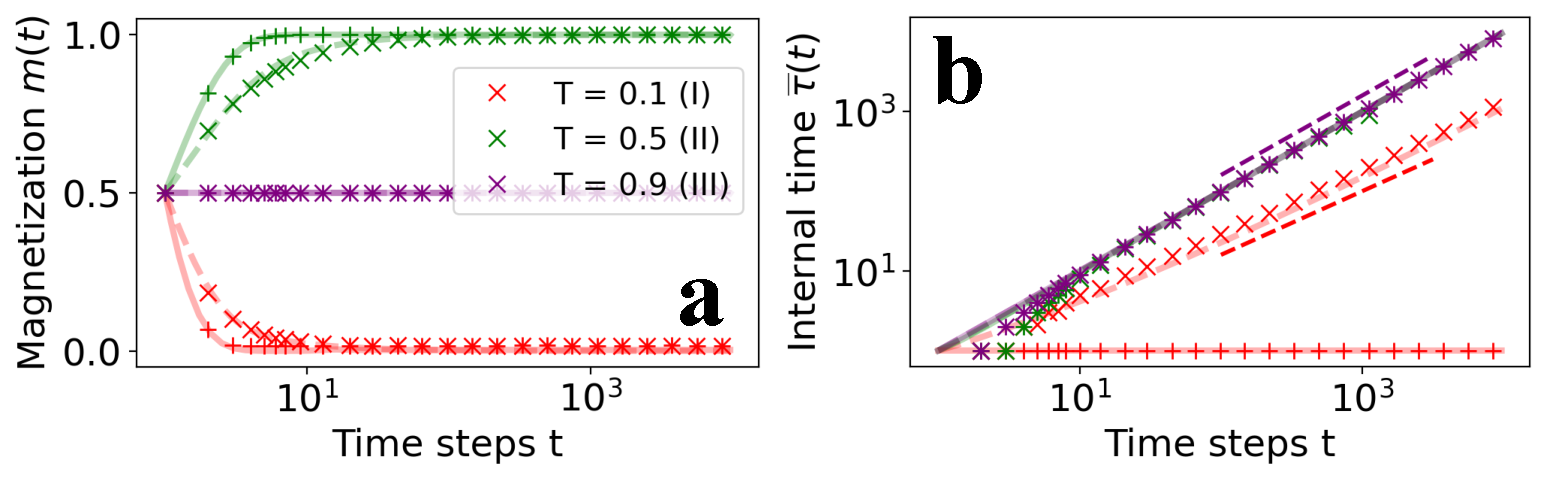
\includegraphics[width=\textwidth]{Figs/Aging_STM/FIG4.pdf}
	\caption[Aging effects in the complete graph]{\label{fig:COM_AGING} Evolution of the average magnetization $m(t)$ \textbf{(a)} and the mean internal time $\bar{\tau}(t)$ \textbf{(b)} in a complete graph of $N=2500$ nodes. Results are shown for the Symmetrical Threshold Model (pluses) and the version with aging (crosses) obtained from simulations. Different colors correspond to different values of the threshold $T$: red ($T = 0.1$) belongs to Phase I, green ($T = 0.5$) belongs to Phase II, and purple ($T = 0.9$) to Phase III. The initial magnetization is fixed at $m_0 = 0.5$. The solid and dashed lines correspond to the numerically integrated solutions from Eq. \ref{eq:HMFaging2} for the original model ($p_A(j) = 1$) and the version with aging ($p_A(j) = 1/(t+2)$), respectively. The dashed lines in (b) show $\bar{\tau}(t) = t$ (purple) and the solution from the recursive relation in Eq. (\ref{eq:RR}) (red). 
	%These expressions are written using a dimensionless time $t$. 
	As computed in Fig. \ref{fig:evolution_random}, for the non-aging version, $\Delta_{m}, \Delta_{\bar{\tau}}  < 4\%$ (except for $T = 0.86$ where $\Delta_{\bar{\tau}} = 10\%$) and for the aging version, $\Delta_{m}^{a}, \Delta^{a}_{\bar{\tau}} < 9\%$ (except for $T = 0.86$ where $\Delta^{a}_{\bar{\tau}} = 15\%$).}
\end{figure}

We note that the dynamical characterization discussed above holds for all possible $m_0$ except for the symmetric initial condition $m_0 = 0$. In this case, an order-disorder transition arises at a critical mean degree $k_c$, whose value depends on the size of the system $N$ \cite{Konstantin}.

\section{\label{sec: Dynamics on a Moore Lattice}  Dynamics on a Moore Lattice}

\begin{figure}
		\centering \captionsetup{font=sf}
		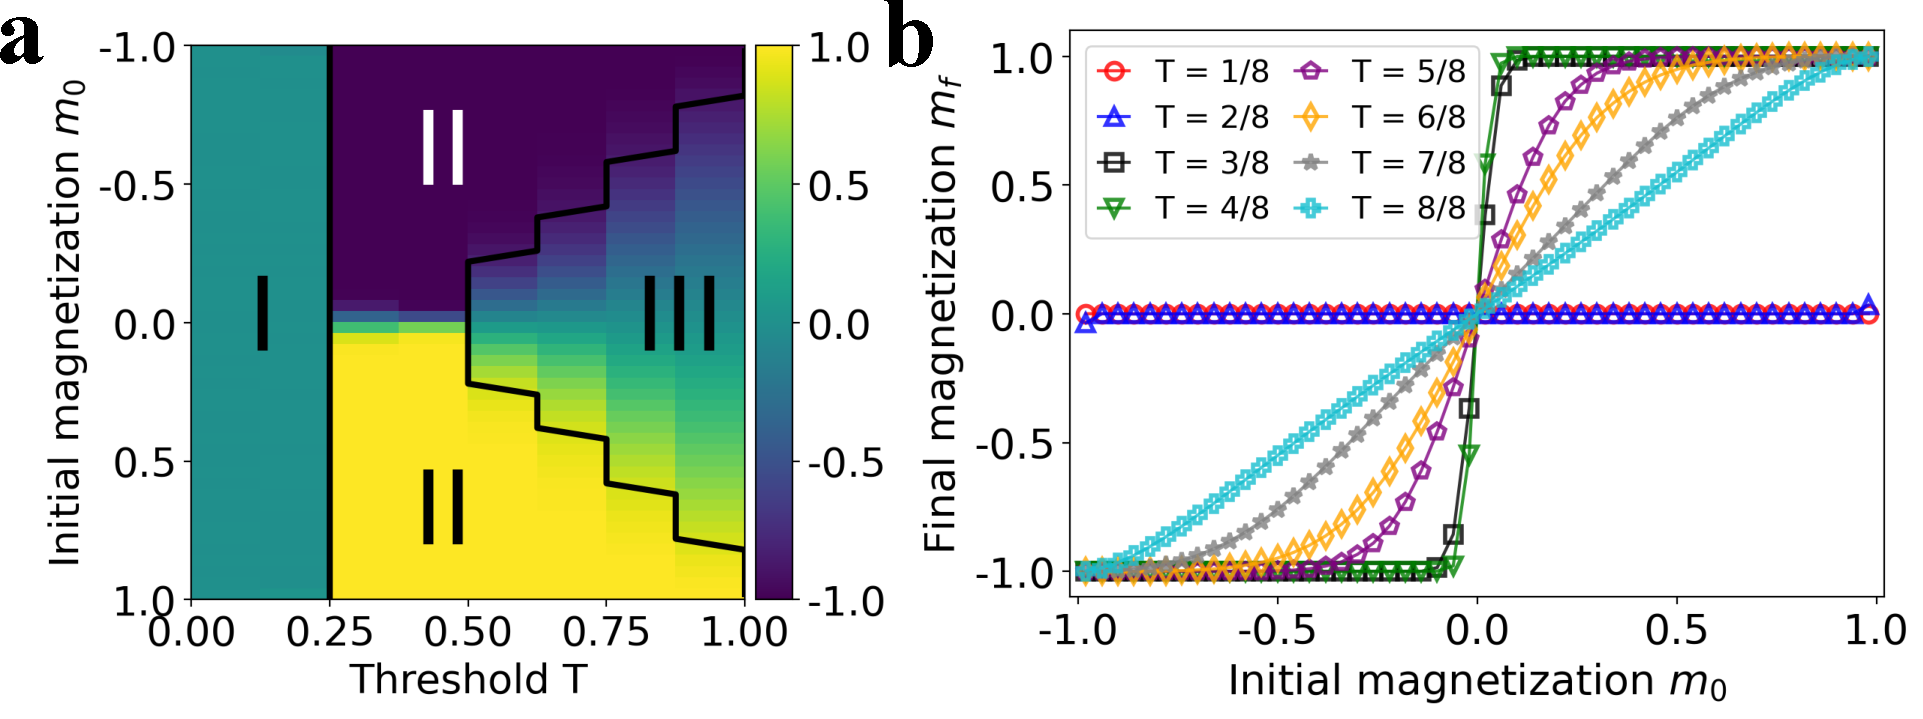
\includegraphics[width=\textwidth]{Figs/Aging_STM/FIG9.pdf}
		\caption[Symmetrical Threshold model in a Moore lattice]{\label{LAT_PD} \textbf{(a)} Phase diagram of the Symmetrical Threshold model in a Moore lattice of size $N = L \times L$, with $L = 100$. The color map indicates the value of the average final magnetization $m_f$. Solid black lines are the borders of Phase II (first and last value of $T$ where the system reaches the absorbing ordered state for each $m_0$), computed from the numerical simulations. \textbf{(b)} Average final magnetization $m_f$ as a function of the initial magnetization $m_0$ for the discrete values of the threshold $T$ (indicated with different colors and markers) in a Moore lattice of the same size. Average performed over 5000 realizations.}
\end{figure}

We consider next the Symmetrical Threshold model in a Moore lattice, which is a regular 2-dimensional lattice with interactions among nearest and next-nearest neighbors ($k=8$).  From numerical simulations, we obtain a phase diagram (Fig. \ref{LAT_PD}a) that is consistent with our previous results in random networks. The system undergoes a mixed-ordered transition at a threshold value $T_{c} = 2/8$  which is independent of the value of the initial magnetization $m_0$. When $T > 4/8$, the system undergoes an ordered-frozen transition at a critical threshold $T_{c}^{*}$, which depends on $m_0$ (similarly to what happens in random networks). The final magnetization $m_f(m_0)$ (Fig. \ref{LAT_PD}b) also shows a dependence on $m_0$ similar to the one found in RR networks (Fig. \ref{ER_REG_PD}c).

\subsection{Original model without aging}

Fig. \ref{fig:evolution_lattice} shows the results from numerical simulations (for $m_0 = 0$ and $0.5$) for the average interface density, the magnetization, and the persistence (the internal time shows the same results as in random graphs). Dynamical properties change significantly for different values of the threshold and initial magnetization $m_0$. Similarly to the case of random networks, we find three different regimes corresponding to the three phases, but with some properties different from the results on  random networks:
\begin{itemize}
	\item \textbf{Mixed regime (Phase I):} It is characterized by fast disordering dynamics with a persistence decay $p(t) \sim \exp(- \ln(t)^2)$, consistent with the results of the Voter model \cite{ben-naim-1996}. The interface density and the magnetization exhibit fast dynamics towards their asymptotic values in the dynamically active stationary state (see $T = 1/8,2/8$ in Fig. \ref{fig:evolution_lattice});
	\item \textbf{Ordered regime (Phase II):} It is characterized by an exponential or power-law decay of the interface density, depending on the initial condition (see details below). The magnetization tends to the absorbing ordered state (see $T = 3/8,4/8$ in Fig. \ref{fig:evolution_lattice});
	\item \textbf{Frozen regime (Phase III):} It is characterized by an initial ordering process, but the system freezes fast (see $T = 5/8$ in Fig. \ref{fig:evolution_lattice}).
\end{itemize}

In particular, in Phase II for $m_0 = 0$ the persistence and interface density decay are found to decay as a power law, $p(t) \sim t^{-0.22}$ and $\rho(t) \sim t^{-1/2}$, respectively (consistent with the results of the Ising model \cite{stauffer-1994,derrida-1995A,derrida-1995B,derrida-1997}). For a biased initial condition ($m_0 = 0.5$), $p(t)$ decays to the initial majority fraction (which corresponds to the state reaching consensus), and $\rho(t)$ follows an exponential-like decay. Note that, for $m_0 = 0$, not all trajectories reach the ordered absorbing states ($m_f=\pm 1$). There exist other absorbing configurations as, for example,  a flat interface configuration for $T = 4/8$, no agent will be able to change, and the system remains trapped in this state. This result is not observed for $m_0 > 0$.

\begin{figure}
		\centering \captionsetup{font=sf}
		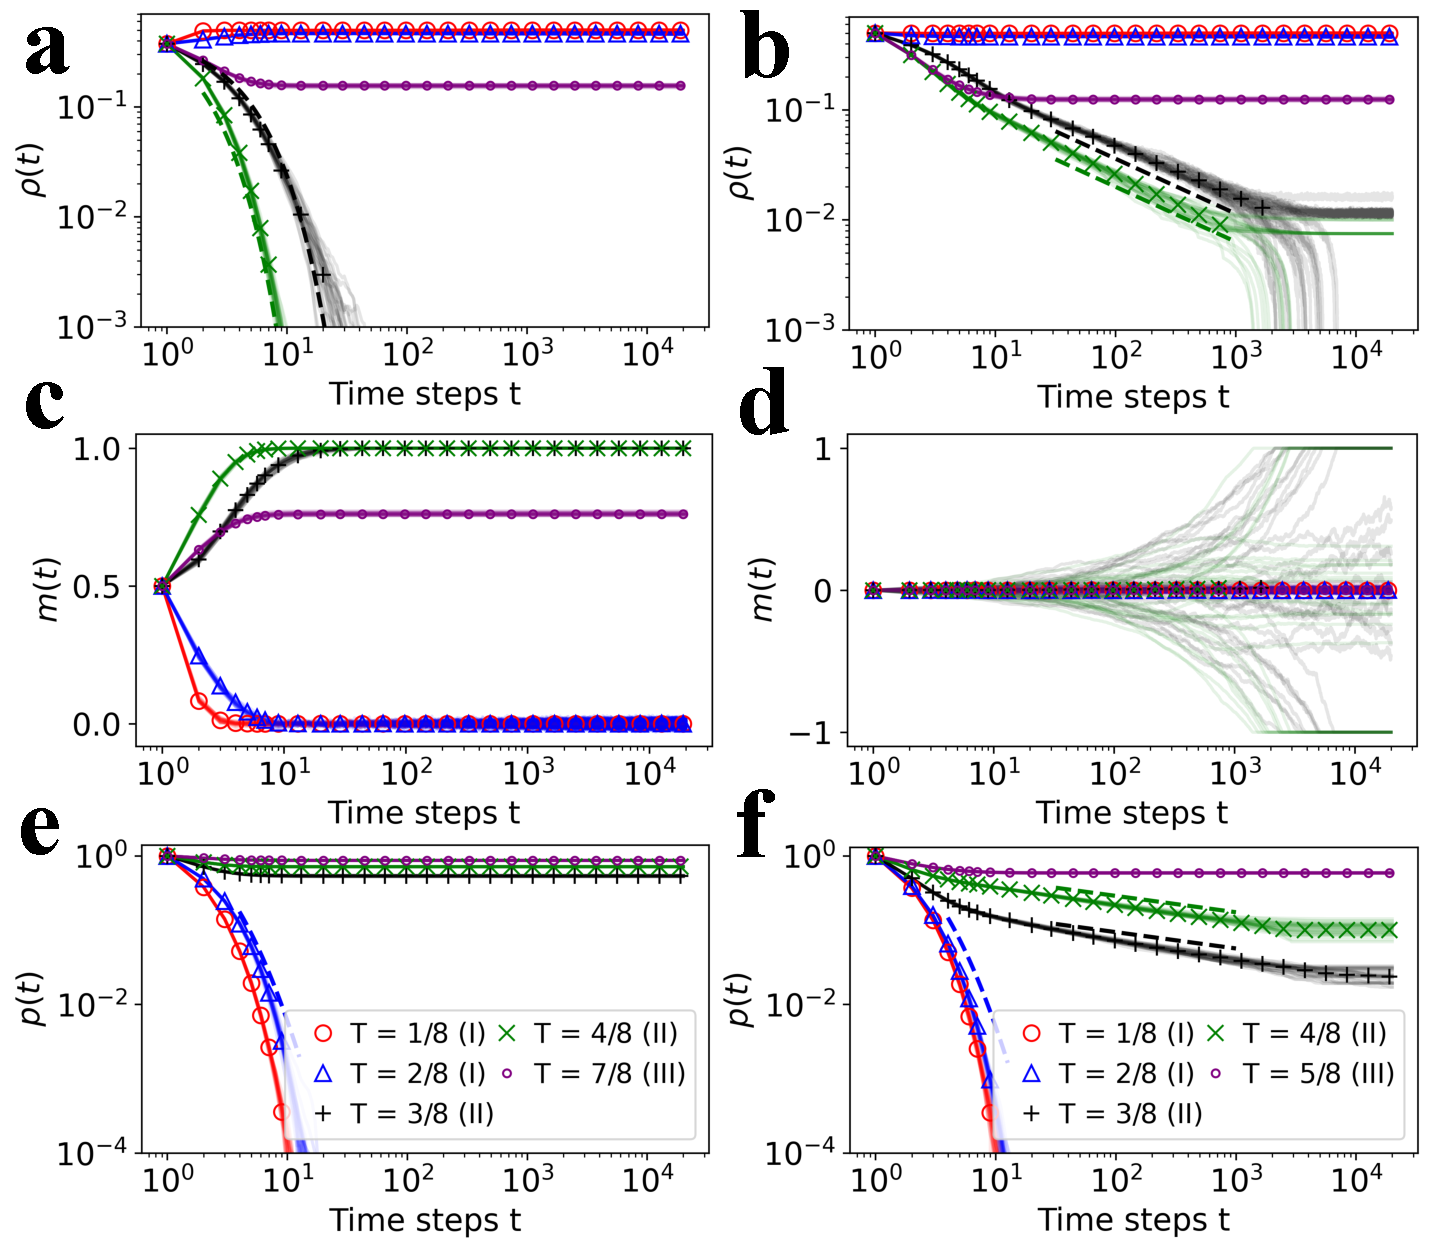
\includegraphics[width=\linewidth]{Figs/Aging_STM/FIG10.pdf}
		%\subfloat[\label{fig:snapshots_model}]{\includegraphics[width=0.8\linewidth]{Figs/Aging_STM/lattice_SGV.png}}
		\caption[Dynamical regimes in a Moore lattice.]{\label{fig:evolution_lattice} Evolution of the average interface density $\rho(t)$ \textbf{(a-b)}, the average magnetization $m(t)$ \textbf{(c-d)}, and the persistence $p(t)$ \textbf{(e-f)} for the Symmetrical model in a Moore lattice starting from a random configuration with $m_0 = 0.5$ (a-c-e) and $m_0 = 0$ (b-d-f). We plot 50 different trajectories in solid lines and the average of $5000$ surviving trajectories (simulations stop when the system reaches the absorbing ordered states) in different markers. Different colors and markers indicate different threshold values: red ($T = 1/8$) and blue ($T = 2/8)$ belong to Phase I, green ($T = 3/8$) and black ($T=4/8$), and purple ($T = 5/8, 7/8$) belong to Phase III. The average magnetization $m(t)$ is computed according to the two symmetric absorbing states. System size is fixed at $N = L \times L$, $L = 200$. The dashed lines in (a) are $\rho \sim \exp(-\alpha \cdot t)$ with $\alpha = 0.5$ (black) and $\alpha = 0.8$ (green), in (b) are $\rho(t) \sim at^{-1/2}$ with $a = 0.36$ (black) and $a = 0.2$ (green), in (e-f) is $p(t) \sim \exp(- \ln(t)^2)$ (blue).
		%These expressions are written using a dimensionless time $t$.
		}
\end{figure}

Contrary, phases I and III show similar dynamics for balanced ($m_0 = 0$) and unbalanced ($m_0 = 0.5$) initial conditions. In Phase I, the system shows disordering dynamics with a persistence decay similar to the one exhibited for the Voter model in a lattice \cite{ben-naim-1996} while in Phase III, the system exhibited freezing dynamics with an initial tendency towards the majority consensus.

Due to the lattice structure and high clustering, the mathematical tools employed in the previous sections for random networks are inapplicable to regular lattices. Consequently, we limit ourselves to the results of numerical simulations. On the other hand, a regular structure facilitates easy modification of the geometry structure of the initial condition. \ref{sec:compact_condition} presents an analysis of how a compact initial condition influences the dynamics of the Symmetrical Threshold model (and its variant with aging).

%For the homogeneous ferromagnetic Ising model on $Z^d$, this probability has been found to decay at large time as a power law $p(t) \sim t^{-\theta(d)}$ \cite{stauffer-1994,derrida-1995A,derrida-1995B,derrida-1997} for $d < 4$. The persistence exponent $\theta(d)$ is considered to be a universal exponent governing non-equilibrium dynamics following a deep quench \cite{majumdar-1996A}. For the pure ferromagnetic Potts model, has been also shown that $p(t)$ decays as a power-law \cite{majumdar-1996B,bray-1994,derrida-1997}. The persistence has also been studied in the context of social dynamics, in particular in the voter model \cite{ben-naim-1996}, where it is shown that the fraction of persistence voters is $p(t) \sim \exp(- \ln(t)^2 )$ in a 2D lattice \cite{ben-naim-1996}.


\section{\label{sec:Summary and Conclusions} Summary and discussion}

In this work, we have studied with Monte Carlo numerical simulations and analytical calculations the Symmetrical Threshold Model. In this model, the agents, nodes of a contact  network, can be in one of the two symmetric states $\pm 1$.  System dynamics follows a complex contagion process in which a node changes state when the fraction of neighboring nodes in the opposite state is above a given threshold $T$. For $T=1/2$, the model reduces to a majority rule or the zero temperature Spin Flip Kinetic Ising Model. When the change of state is only possible in one direction, say from $1$ to $-1$, it reduces to the Granovetter-Watts Threshold model \cite{granovetter-1978,watts-2002,Abella-2022-AME}. We have considered the cases of a fully connected network, Erd\H{o}s-Rényi, and random regular networks, as well as a regular two-dimensional Moore lattice. 

We have found that, in the parameter space of threshold $T$ and initial magnetization $m_0$, the model exhibits three distinct phases, namely Phase ${\rm I}$ or mixed, Phase ${\rm II}$ or ordered, and Phase ${\rm III}$ or frozen. The existence of these three phases is robust for different network structures.
% and the mixed-ordered and ordered-frozen transitions show nontrivial dependence on the threshold and the initial magnetization ($T_{c}(m_0)$ and $T_{c}^{*}$). 
These phases are well characterized by the final state ($m_f$), and by dynamical properties such as the interface density $\rho(t)$, time-dependent average magnetization $m(t)$, persistence times $p(t)$, and mean internal time $\bar{\tau}(t)$. These phases can be obtained analytically in the mean-field case of a fully connected network. For the random networks considered, we derive an approximate master equation (AME) \cite{gleeson-2013,Abella-2022-AME} considering agents in each state according to their degree $k$,  neighbors in state $-1$, $m$, and age $j$. From this AME, we have also derived a heterogeneous mean-field (HMF) approximation. While the AME reproduces with great accuracy the results of Monte Carlo numerical simulations of the model (both static and dynamic), the HMF shows an important lack of agreement, highlighting the importance of high-accuracy methods necessary for threshold models. 

%For the random networks studied, we derived a mathematical description based on approximate master equation and am heterogeneous mean-field approximation. We found that, as it occurred for the Watts' threshold model, the HMF approximation is not enough to describe the full phase diagram, even though it captures qualitatively the mixed-ordered transition. On the other hand, the full AME gives a good description of the full phase diagram for the networks studied here, even though it has a high computational cost. Regarding the dynamics, from our AME numerical solution we extracted the information about the magnetization, the interface density and the persistence. While for $m(t)$ and $p(t)$ the AME matches the numerical simulations with great accuracy, for $p(t)$ the AME description does not match the results from numerical simulations. We associate this error to the finite size effects, which are more relevant for this magnitude.

%Aging is incorporated as a resistance to state change that is inversely proportional to the persistence time.
Aging is incorporated in the model as a decreasing probability to modify the state as the time already spent by the agent in that state increases. The key finding is that the mixed phase (Phase ${\rm I}$), characterized by an asymptotically disordered dynamically active state, does not always exist: the aging mechanism can drive the system to an asymptotic absorbing ordered state, regardless of how low the threshold $T$ is set. A similar effect of aging was already described for the Schelling model in Ref. \cite{Abella-2022}. When the dynamics are examined in detail, a new Phase ${\rm I}^{*}$, defined in terms of dynamical properties, emerges in the domain of parameters where the model without aging displays Phase ${\rm I}$. This phase is characterized by an initial disordering regime ($m \to 0$) followed by a slow ordering dynamics, driving the system toward the ordered absorbing states (including the one with spins opposite to the majoritarian initial option). This result is counter-intuitive since aging incorporates memory into the system, yet in this phase, the system ``forgets'' its initial state. The network structure plays an important role in the emergence of Phase ${\rm I}^{*}$ since it does not exist for complete graphs. A detailed analysis reveals that Phase ${\rm I}^{*}$ replaces Phase ${\rm I}$ only for sparse networks, including the case of the Moore lattice. For ER networks we find that, as the mean degree increases, Phase ${\rm I}$ reappears and there is a range of values of the mean degree for which phases ${\rm I}$ and ${\rm I}^{*}$ coexist. Beyond a critical value of the mean degree, Phase ${\rm I}$ extends over the entire domain of parameters where Phase ${\rm I}^{*}$ was observed.

While aging favors reaching an asymptotic absorbing ordered state for low values of $T$ (Phase ${\rm I}$), in Phase II the ordering dynamics are slowed down by aging, changing, both in random networks and in the Moore lattice, the exponential decay of the interface density by a power law decay with the same exponent. The aging mechanism is found not to be important in the frozen Phase ${\rm III}$. All these effects of aging in the three phases are well reproduced for random networks by the AME derived in this work, which is general for any chosen activation probability $p_A (j)$.

For the Moore lattice, we have also considered in detail the special case of the initial condition $m_0=0$. In this case, Phase ${\rm I}^{*}$ emerges, and Phase ${\rm III}$ is robust against aging effects. However, in Phase ${\rm II}$ aging destroys the characteristic power law decay of the interface density, $\rho(t) \sim at^{-1/2}$, associated with curvature reduction of domain walls. This would be a main effect of aging in the dynamics of the phase transition for the zero temperature spin flip Kinetic Ising model \cite{gunton1983}. Additionally, this regular structure allowed us to analyze the effects of a compact initial condition. We have shown that the joint effect of aging and a compact initial condition prevent the ordered phases from reaching the consensus state (see \ref{sec:compact_condition}).

As a final remark on the general effects of aging in different models of collective behavior, we note that the replacement of a dynamically active disordered stationary phase by a dynamically ordering phase is generic. In this paper, we find the replacement of Phase ${\rm I}$ by Phase ${\rm I}^{*}$. Likewise in the Voter model, aging destroys long-lived dynamically active states characterized by a constant value of the average interface density, and it gives rise to coarsening dynamics with a power law decay of the average interface density \cite{fernandez-gracia-2011}. In the same way, in the Schelling segregation model, a dynamically active mixed phase is replaced, due to the aging effect, by an ordering phase with segregation in two main clusters. 
Another aging effect that seems generic, in phases in which the system orders when there is no aging, is the replacement of dynamical exponential laws by power laws. This is what happens here in  Phase ${\rm II}$ for the decay of the average interface density but, likewise, exponential cascades in the Granovetter-Watts model are replaced due to aging by a power-law growth with the same exponent \cite{Abella-2022-AME}.

Further research with the general AME used in this study would involve a new approach that considers the master equation, as described in Ref. \cite{peralta-2020B}. This approach aims to incorporate finite size effects, which are relevant when $m_0$ is close to zero, and would provide a mathematical framework for further analyisis of the results in Ref. \cite{Konstantin}. Regarding the model, this article reports the main features of the Symmetrical Threshold model dynamics and the aging effects. However, there are several areas for future research along this lines, such as investigating the impact of strongly heterogeneous \cite{barabasi2009scale} or coevolving networks \cite{Zimmermann,vazquez-2008}, exploring the dependence of the results on the aging activation function $p_A$, and examining the joint effect of aging and strongly heterogeneous degree distributions.